\documentclass[a4paper,titlepage]{ltjsarticle}
\usepackage{luatexja} 

\usepackage{amsmath, amssymb, ar, bm, booktabs, siunitx, url, graphicx, multirow, xurl, enumerate, longtable, mathtools, pxrubrica, comment, ascmac, fancybox}

\usepackage{here}

\newcommand{\hang}[1]{%
	\settowidth{\hangindent}{#1}%
	#1%
}%


\newenvironment{hangall}[1]{\hangindent = #1zw\everypar{\hangindent = #1zw}}{}

\graphicspath{{picture}}

\begin{document}

\title{航空工学実験Ⅰ \\流れの観察法}
\author{2班 2年 2020番 大村蒼摩}
\date{実験日:7月4日\\審査日:7月11日\\再提出日:7月25日}
\maketitle

\setlength{\abovedisplayskip}{15pt} 
\setlength{\belowdisplayskip}{15pt}

\tableofcontents
\clearpage

\vskip\baselineskip

\section{概要}
今回の実験では,流体現象の計測法,観察法,物体まわりの
流れを正しく理解するために,電動機の回転数と測定部の
風速の測定,円柱周りの圧力分布の測定,流れの可視化の
3つの実験を行った.そこから回転数と風速には比例関係
があることや,圧力分布から剥離点の角度の測定,物体形状
と剥離領域の関係などについて考察した.

\section{目的}
本実験では,風洞実験を通じて流体現象の計測法と観察法を
習得し,それらを基礎に物体まわりの流れを正しく理解する.

\section{理論}
\subsection{$粘性^{[6]}$}
流れを解析する際に重要な物性.流体が変形を受けるときに抵抗する性質で,流れに摩擦が生じ,流れの損失や流体中の運動する物体の抵抗の原因となるもの.

\begin{figure}[hbtp]
  \centering
  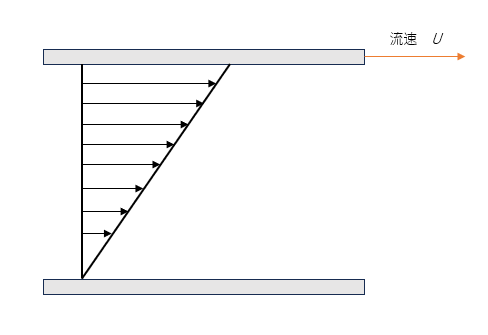
\includegraphics[height=5cm,width=8cm]{nagare2.png}
  \caption{クエット流れ}
  \label{クエット}
\end{figure}

\subsection{$境界層^{[8]}$}
  固体壁に沿う流れを,粘性の影響が及ぶ固体壁近傍の流れと,その外側の流れに分けて考え,前者の流れの領域のことを境界層という.境界層内では粘性のため渦が生成され,流れの運動エネルギーが熱エネルギーに変換され損失が生じる.
  また,速度$U$の一様流れ中に置かれた平板上に形成される境界層を考えると,境界層は平板先端から下流に向かうにつれて発達する.先端付近の境界層内の流れは平板に沿って層をなして流れており,このような境界層を層流境界層という.しかし,あるところから下流では境界層内の流れはランダムに変動する乱れた流れになる.このような境界層を乱流境界層という.


\subsection{$剥離^{[3]}$}
 物体表面に形成された境界層は流れの方向に厚さを増加させながら流れていき,表面が凸形状になっていると下流において圧力が増加し,境界層の中でも圧力が増加していく.
 物体の表面上の流れは粘性力の影響で両側が遅くなりので,下流に向かって流れていくことができなくなる.このようなことより,図3のように反対方向に流れる.
 また完全流体では,円柱の周りの流れは上下左右対称となり,境界層は発生しない.
 この場合,円柱表面での圧力は次のようになる.
 
 \begin{equation}
  C_P=1-4\sin^2\theta
 \end{equation}

\begin{figure}[hbtp]
  \centering
  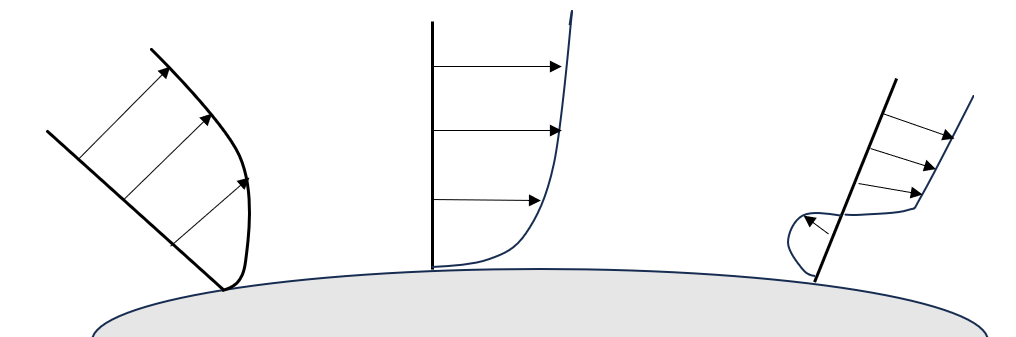
\includegraphics[height=5cm,width=8cm]{nagare3.png}
  \caption{円柱周りの剥離}
  \label{剥離}
\end{figure}


\subsection{$風洞の種類,特徴^{[4]}$}
\subsubsection{低速風洞}
 低速風洞は開放型と回流型の二つに分類できる.
開放形風洞はエッフェル形と呼ばれ,吸入口と吹出し口が
大気に直接開放されているのが特徴である.この構造の風洞は,
一定の風速における必要動力が大きいという欠点がある.
一方で,同じ空気を循環していないか,あるいは部屋の広さが
広いがゆえに,煙による流れの可視化実験のときは,長時間運転
させることが可能である.
回流形はゲッチング型と呼ばれ,空気変換器をつけていない限り,
同じ空気を循環させるため,動力は小さくなる.さらに,回流形は
二つに分けることが可能である.単帰路式と複帰路式だ.単帰路式
では送風機部の風路が1本であるが,複帰路式は2本必要になる.

\subsubsection{超大型風洞}
 超大形低速風洞の目的はレイノズル数の効果を緩和するために,実機を供試体として
 実験することだ.特徴は,名前からわかる通り,ほかの風洞に比べて超大形という
 ことだ.カリフォルニア州のNASA Ames研究所の風洞は12.2m×24.4mと24.4m×36.6mの
 風洞がある.この風洞は最大風速134m/s出すことができる.この風洞に必要な動力は
 100670kWである.

\subsubsection{高レイノルズ数}
 風洞実験において高レイノルズ数を得るために,測定部内の空気の密度を上げる方法
 が長年利用されている.NASAにある高レイノルズ数は,実験気圧を最大20気圧まで
 圧縮することが可能である.また,液体窒素を噴射状にして風路内の空気と混合させ、
 低温にすることで高レイノルズ数を得る方法もある.このような風洞ではマッハ0.2
 からマッハ1.2の範囲で運転が可能である.

\subsubsection{V/STOL用風洞}
 V/STOL機は,一般航空機に比べて吹下し角が大きく,汎用風洞測定部では壁干渉が
 大きくなり,好ましくない.そのため,壁干渉を軽減するように測定部を一段と
 大きくしたものである.

\subsubsection{突風風洞}
 測定部の風上に正弦波の突風を発生させる装置がある.一連の翼を機械的に
 振動することによって任意の周期と振動を持った突風が得られる.航空機の
 突風応答実験に用いられる.

 \subsubsection{アイシング風洞}
 翼の前縁,エンジンインレットなどにおける氷結状態および防除氷装置の効果を
 実験する風洞実験である.

 \subsubsection{環境用試験用風洞}
  大気拡散問題の研究,建築構造物の風圧特性の実験,風害,台風災害対策の
 実験などに用いられる.

 \subsection*{ピトー静圧管}
 \begin{itemize}
  \item ピトー静圧管は圧力計と組み合わせて使うことで,動圧を計測する装置である.
  \item ピトー管の総圧:$p_0$,静圧:$p_\infty$,動圧:$q=\frac{\rho U^2}{2}$とするとベルヌーイの法則より風速:$U$は次式のように書くことができる.実際に実験では$p_0-p_\infty$を計測している.
  \begin{align}
    p_0&=p_\infty+q=p_\infty+\frac{\rho U^2}{2}\\ 
    U&=\sqrt \frac{2(p_0-p_\infty)}{\rho }
  \end{align}
 \end{itemize}

 \subsection{風洞実験での圧力の計測方法}
 模型の表面に多数の測圧孔を規則正しく分布して,この孔にかかる圧力を測定する.
 方法としては,模型内部でチュービングまたは管を使って,孔からの圧力測定器具
 につないで測定を行う.ただし,模型表面の測圧孔の周りは,突起物,まくれが
 無いように注意する.

\subsection{$流れの可視化_{[9]}$}
流れの可視化することの利点は,1枚の写真から広い流れの場の空間的に構造が
瞬間的に手威力的に得られること.同じ量の情報を流れの可視化以外の方法で
得るのは難しい.短所は,圧力や渦度に関する情報を直接的には得ることが
困難なこと.

\subsection{円柱周りの流れ}
円柱周りの流れは,層流境界層が形成される場合と乱流境界層が形成される場合がある.
レイノズル数が$2.0\times10^{5}$以下の流れのとき,円柱表面には層流境界層が形成され,
剥離点は前方にあって剥離領域は大きく,その結果円柱が受ける抗力は大きくなる.
レイノズル数が$4.2\times10^{5}$以上の流れのとき,境界層は乱流境界層になり,剥離点が
後退し,剥離領域も小さくなっている.その結果,円柱の受ける抗力は小さくなる.
また,物体後方に互い違いに形成された渦列をカルマン渦列という.
これは円柱にだけ発生する現象ではなく,流れに平行な平板のように剥離のない
物体の後流でも形成される.つまりは,後流の不安定さで形成されるかが決まる.

\section{実験手順}
実験中に,実験装置のスケッチ又は写真撮影を行う.また,実験中に風洞周辺で
起きた事象は実験結果へ影響する場合があるので,詳細に記載する.
このとき,模型の取り付け位置,ピトー静圧管の直径を測定する.

\subsection{電動機の回転数と測定部の風速}
風洞の計測可能風速範囲を計測する.
\begin{enumerate}
  \item 実験室内の大気圧・気温・湿度(気象条件)を計測する.
  \item 計測器の初期設定を行う.
  \item 送風機の回転数を変えながら,動圧と風速を計測する.
  \item 実験室内の大気圧・気温・湿度を計測する.
\end{enumerate}

\subsection{円柱の圧力分布}
円柱の圧力分布を計測する.風洞の閉塞率を確認する.
\begin{enumerate}
  \item 実験室内の大気圧・気温・湿度を計測する.
  \item 計測器の初期設定を行う.
  \item 送風機の回転数を設定し,動圧と風速を計測する.
  \item 円柱を時計回りに回転させ,0{\textdegree}から180{\textdegree}まで10{\textdegree}おきに変化させる.
  \item それぞれの角度において,円柱表面の圧力と変動率を計測する.その際,PCに表示されている圧力の変動なども同時に観察する.
  \item 計測を行いながら,同時に剥離点の推定を行う.圧力の変動から推定できる.
  \item 実験室の大気圧・気温・湿度を計測する.
  \item 計測後,適切な圧力分布が得られたかどうかを計測結果から判断する.
\end{enumerate}



\subsection{物体まわりの流れの可視化}
円柱,角柱,二次元元翼について流れの可視化を行う.
\begin{enumerate}
  \item 各模型の代表長さを計測する.
  \item 実験室内の大気圧・気温・湿度を計測する.
  \item 計測器の初期設定を行う.
  \item 煙の流れがよく見えるように送風機の回転数を設定し,動圧と風速を計測する.
  \item 物体まわりの流れを可視化した写真を撮影する.このとき,撮影位置,方向、角度,などを固定して撮影を行い,必要であれば三脚を使用する.
  \item 煙の線が意味する現象,煙の線お形状から何が分かるのかを考察しながら観察する.
  \item 模型形状の影響を観察する.鈍頭物体,竜泉物体の相違など.
\end{enumerate}

\subsection{円柱の抗力係数の推算}
\begin{enumerate}
  \item 圧力係数の計算\\
  測定された円柱表面の圧力差$P-P_{\infty}$をそれぞれの角度で無次元化し,
  圧力係数$C_{P}$とする.圧力係数は次式で定義される.

  \begin{equation}
c_p=\frac{p-p_\infty}{Q}=\frac{p-p_\infty}{\frac{\rho U^2}{2}}    
  \end{equation}

  \item 円柱の抵抗係数$C_P$は次式によって求められる.
  この$C_P$は圧力による抵抗係数で,圧力抵抗係数または
  形状抗力係数と呼ばれる.
  \begin{equation}
      C_D=\frac{\int _Sp\cos \theta dA}{\frac{\rho U^2S}{2}}=\frac{\pi}{180}\int_{180}^{0} C_p \cos \theta d\theta 
      \label{cd}
  \end{equation}

\end{enumerate}

 ここで,表面積:$S$,傾きを考慮した面素:$A$である.また,
\theta は弧度法でなく度数法で表記される.また,実際の流れでは,
常識の解析的な積分が行えない.そのため,
この式を用いるため,まず$\ang{10}$刻みの各$C_P$から$C_P cos\theta$
を計算する.そして、以下の2通りの方法で$C_D$を数値積分に
より算出する.
\begin{enumerate}
  \item 台形法により数津積分して,$C_P \cos\theta$から$C_D$
  を求める
  \item シンプソンの公式により数値積分して,$C_p \cos\theta$
  から$C_D$を求める.
\end{enumerate}
一般に,抵抗係数$C_D$はレイノルズ数が$Re$に対して表される.
\\
\\
\section{実験装置}

\begin{figure}[hbtp]
  \centering
  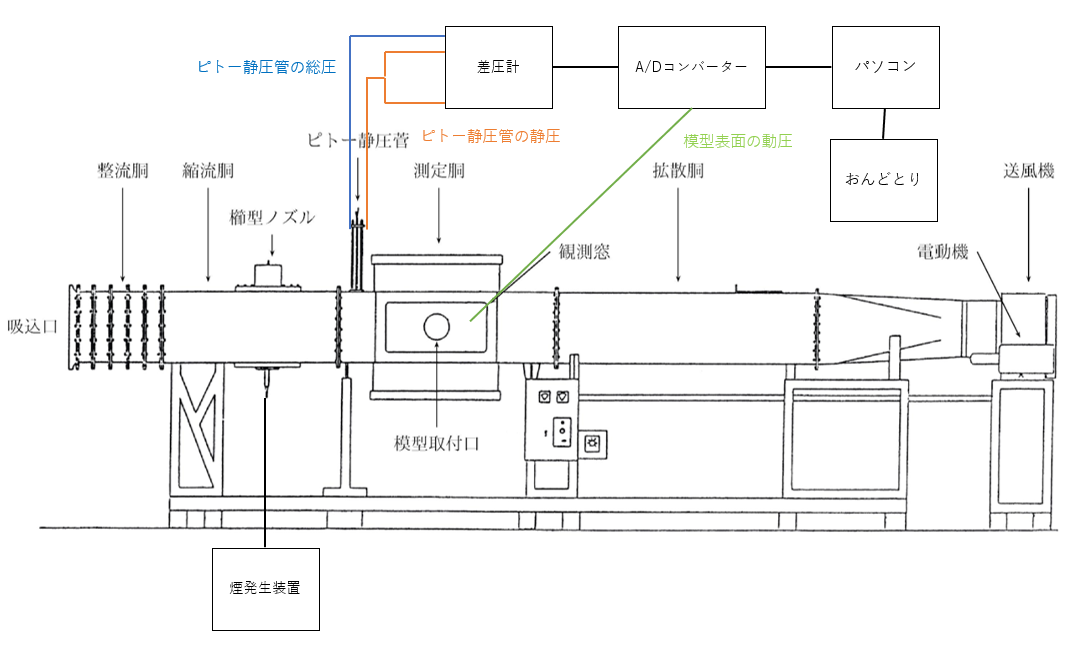
\includegraphics[width=15cm]{風洞.png}
  \caption{実験装置の簡略図}
  \label{簡略図}
\end{figure}

\clearpage

\subsection{風洞}

\begin{figure}[hbtp]
  \centering
  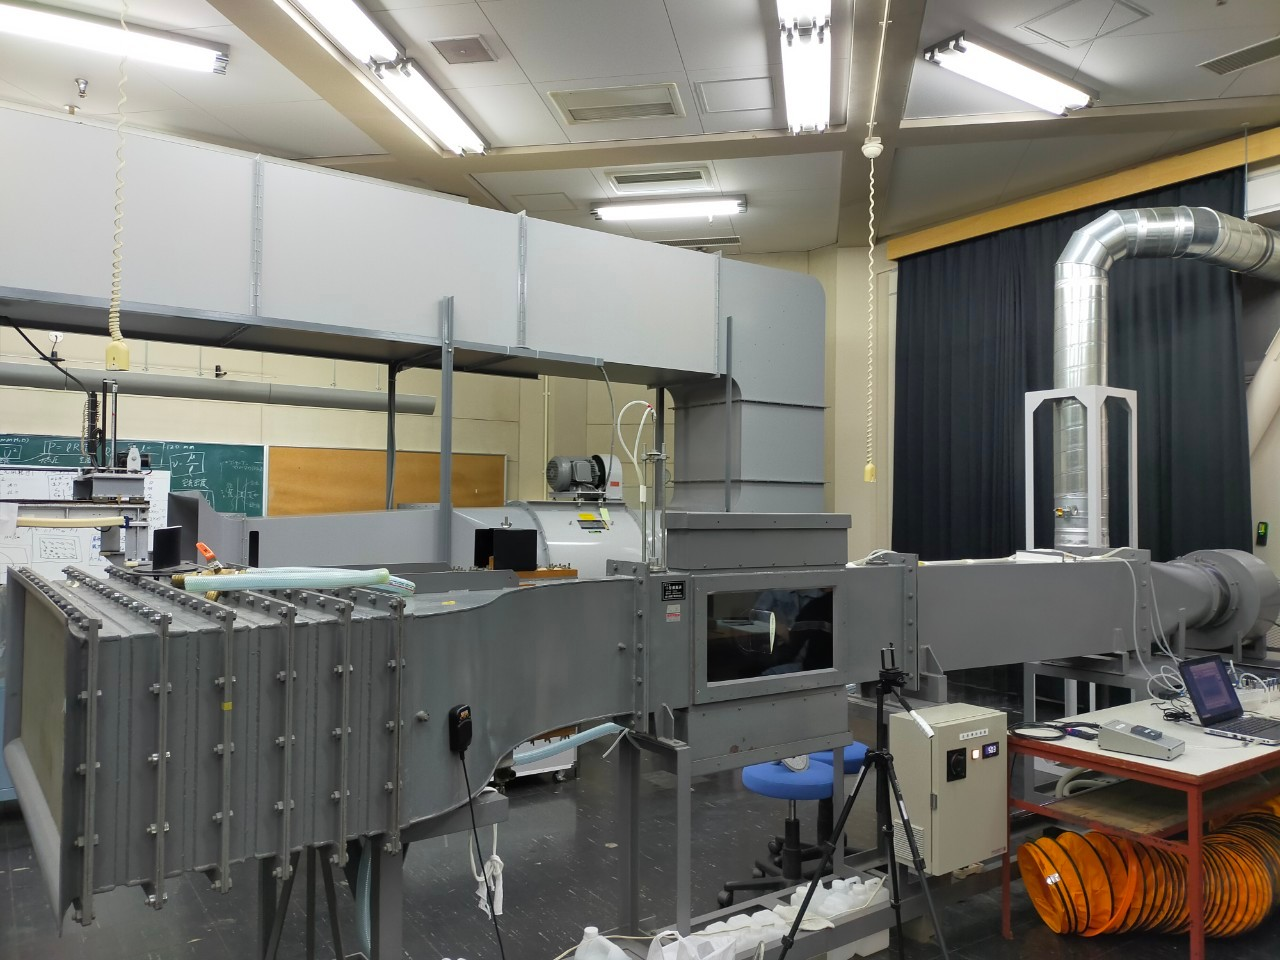
\includegraphics[width=6cm]{風洞全体図.jpg}
  \caption{風洞}
  \label{風洞}
\end{figure}


\begin{table}[hbtp]
  \caption{風洞}
  \centering
  \begin{tabular}{cc}
    \toprule
    風洞&\\
    \hline
    形式 & 吸込2次元煙風洞\\
    
    縮流比 & 12:1\\
    
    ダイピングスクリーン & 20メッシュ 6枚\\
    
    観測部 & 長さ 1250mm 高さ400mm 幅 100mm\\
    
    観測部窓 & 幅 600mm 高さ300mm\\
    
    送風機 & 50{\si{m^3/min}}\\
    
    風速 & 2.145~14.562{\si{m/s}}\\
    
主流流れ & 未計測{\si{m/s}}\\
\bottomrule
  \end{tabular}
\end{table}

\clearpage

\subsection{電動機・制御盤}

\begin{figure}[hbtp]
  \begin{minipage}[b]{0.45\linewidth}
    \centering
    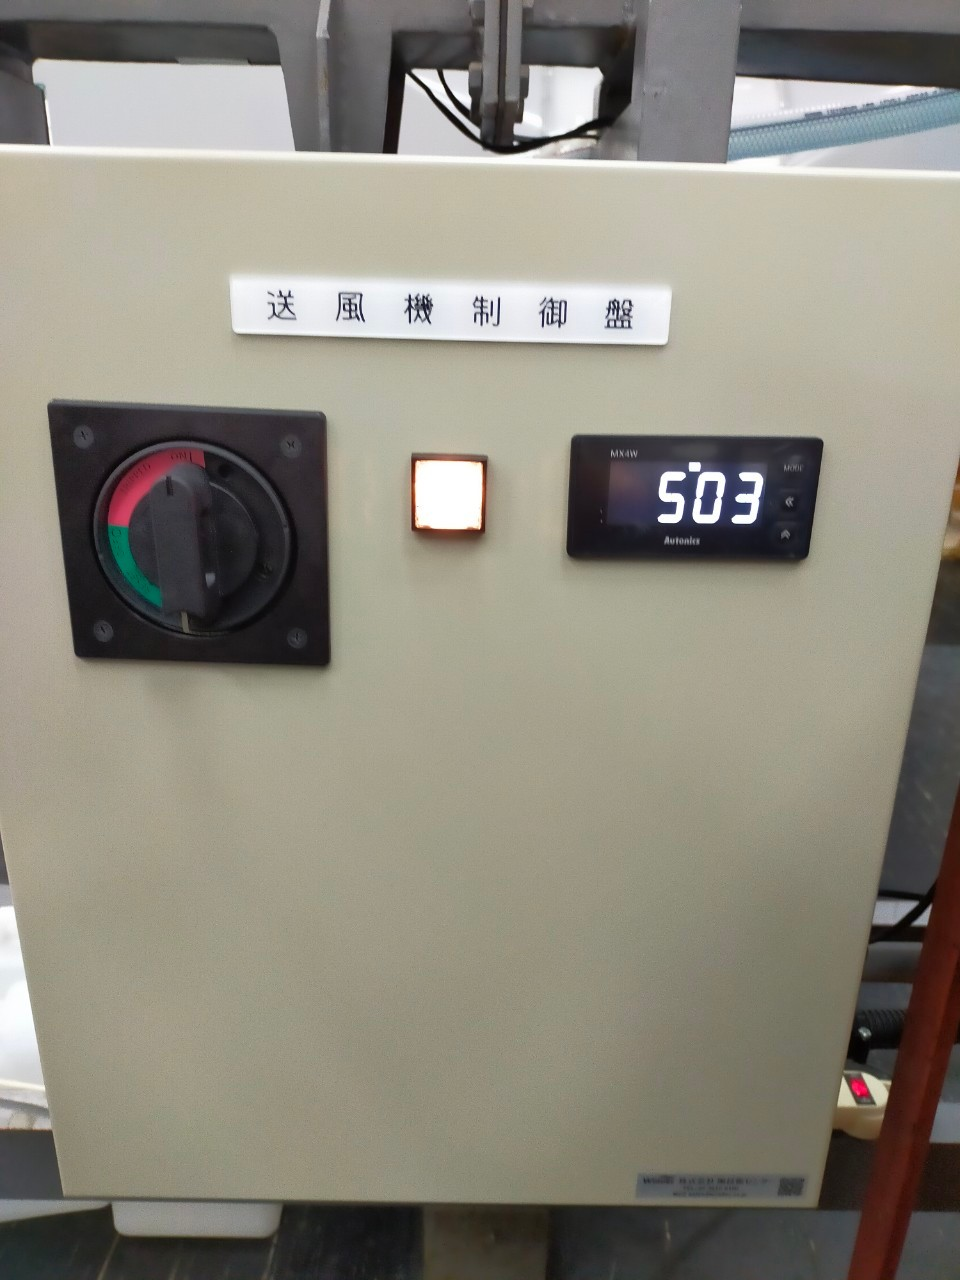
\includegraphics[width=6cm]{制御盤.jpg}
    \caption{制御盤}
    \label{制御盤}
  \end{minipage}
  \begin{minipage}[b]{0.45\linewidth}
    \centering
    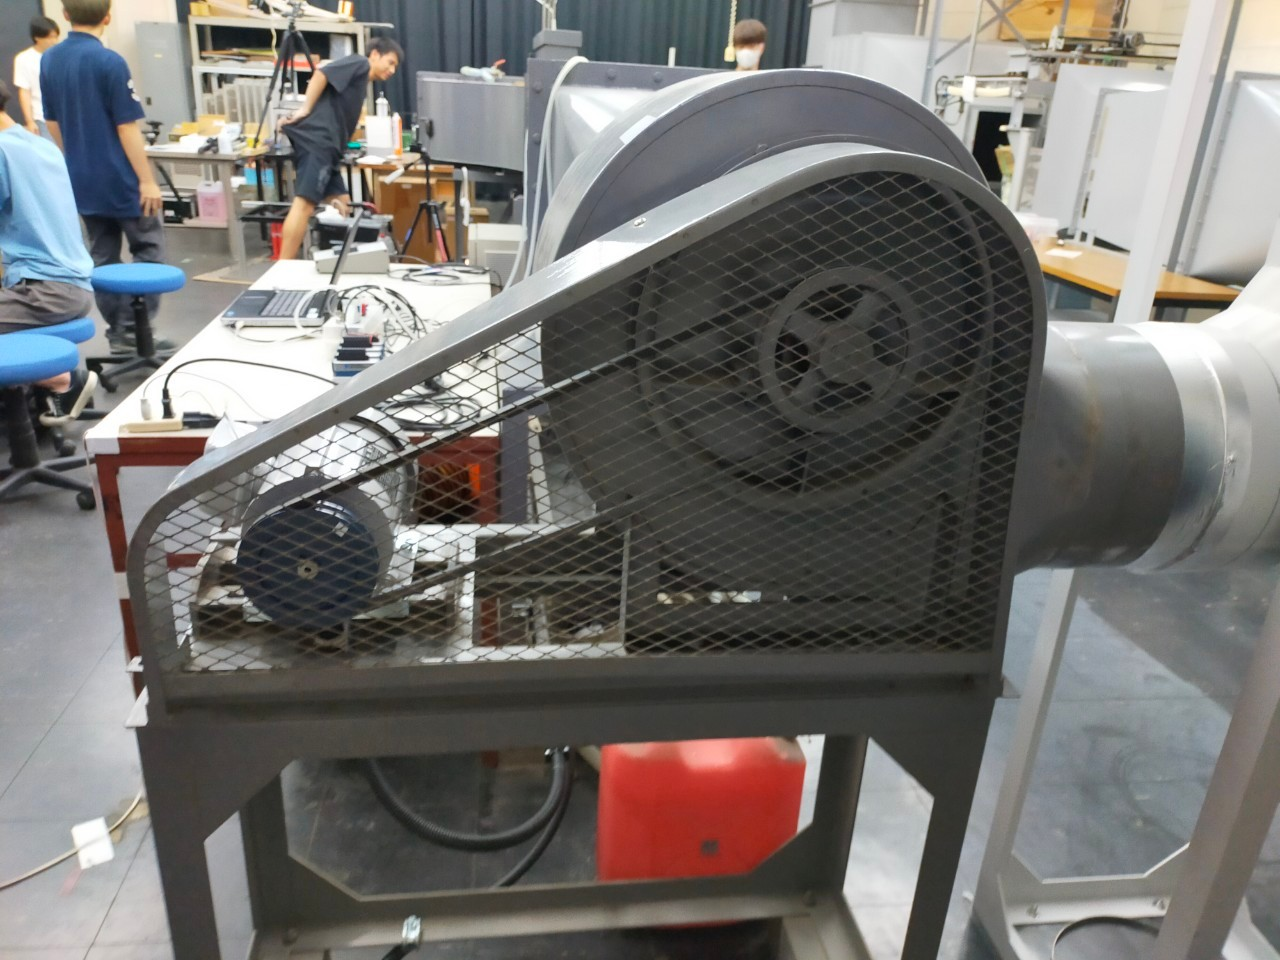
\includegraphics[width=6cm]{電動機.jpg}
    \caption{電動機}
    \label{電動機}
  \end{minipage}
  \end{figure}


\begin{table}[hbtp]
  \caption{電動機・制御盤}
  \centering
  \begin{tabular}{cc}
    \toprule
    電動機・制御盤 &\\
    \hline
    制御方式 & 誘導モータ+インバータ制御\\
    
    電動機 & 0.75{\si{kW}} 4$P$ 3\phi 200{ \si{V} }全閉外扇\\
    
    インバータ & ファン・ポンプ用インバータ 0.75{\ si{kW}} 3\phi 200{ \si{V}}\\
    
    \multirow{2}{*}{制御盤} & 電源ブレーカハンドル・設定用回転数表示機能・操作パネルボックス\\
   & (本体寸法:H500$\times$W400$\times$D200 \divideontimes 凸部除く)\\
    通信 & RS485(4線式)\\
    \bottomrule
  \end{tabular}
\end{table}

\clearpage

\subsection{煙発生装置}
\begin{figure}[hbtp]
  \centering
  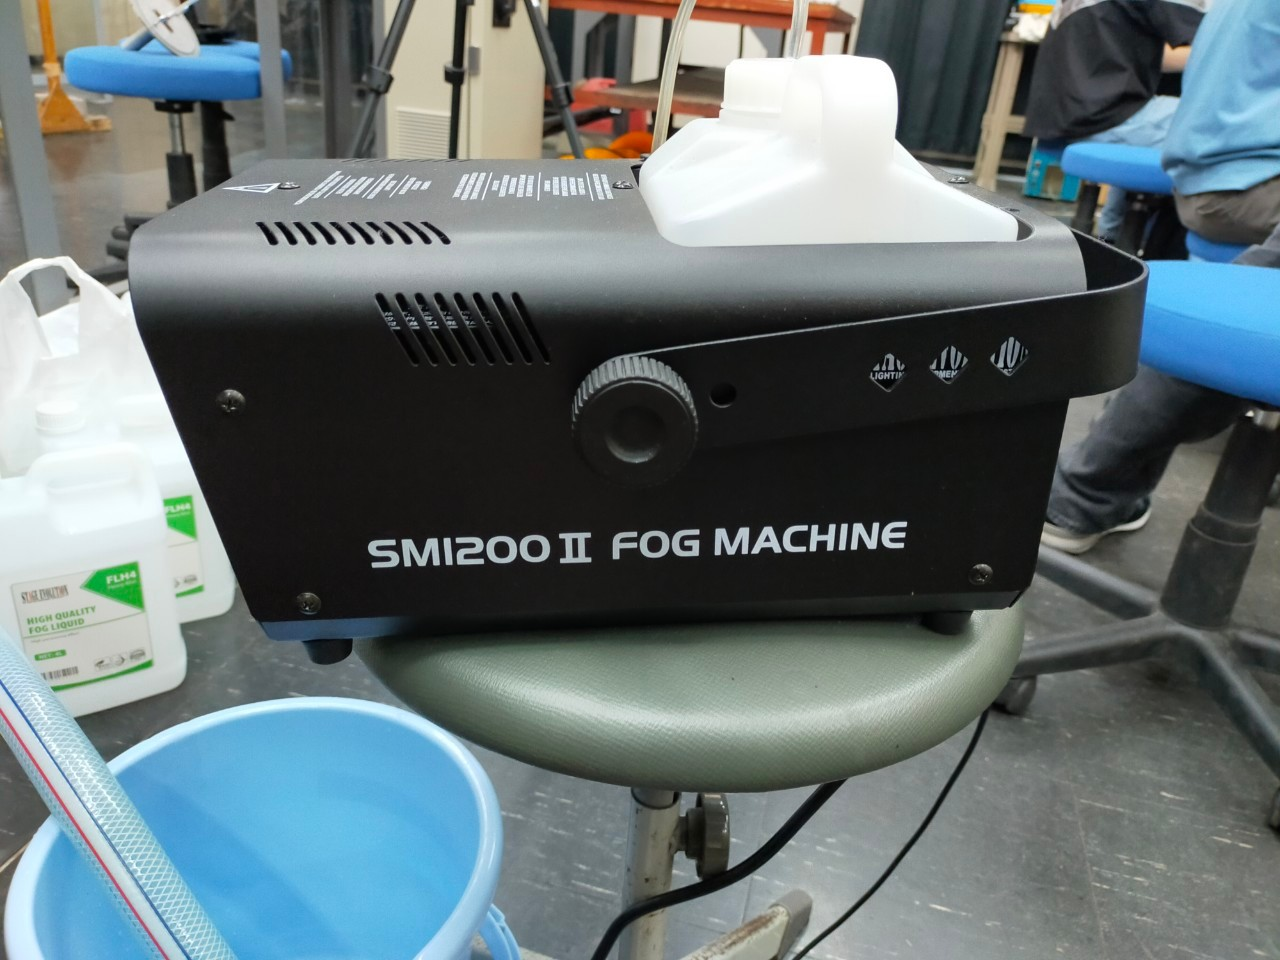
\includegraphics[width=6cm]{煙発生装置.jpg}
  \caption{煙発生装置}
  \label{煙}
\end{figure}

\begin{table}[hbtp]
  \caption{煙発生装置}
  \centering
  \begin{tabular}{cc}
    \toprule
    煙発生装置\\
    \hline
    メーカー/製品名 & STAGE EVOLUTION /SN1200Ⅱ\\
  ヒーターパワー & 1100{ \si{W}}\\
  ウォームアップ & 8{ \si{min}}\\
  フォグ容量 & 198{ \si{m^3/min}}\\
  タンク容量 & 2.5{ \si{L}}\\
  電源電圧 & AC100{ \si{V}}\\
  煙導構造 & 翼型導管構造\\
  ノズル間隔 & 25{ \si{mm}}\\
  ノズル径 & \phi 1.2~1.4{ \si{mm}}\\
  ノズル数 & 40本\\
  \bottomrule
  \end{tabular}
\end{table}

\clearpage

\subsection{計測器}

\begin{figure}[hbtp]
\begin{minipage}[b]{0.45\linewidth}
  \centering
  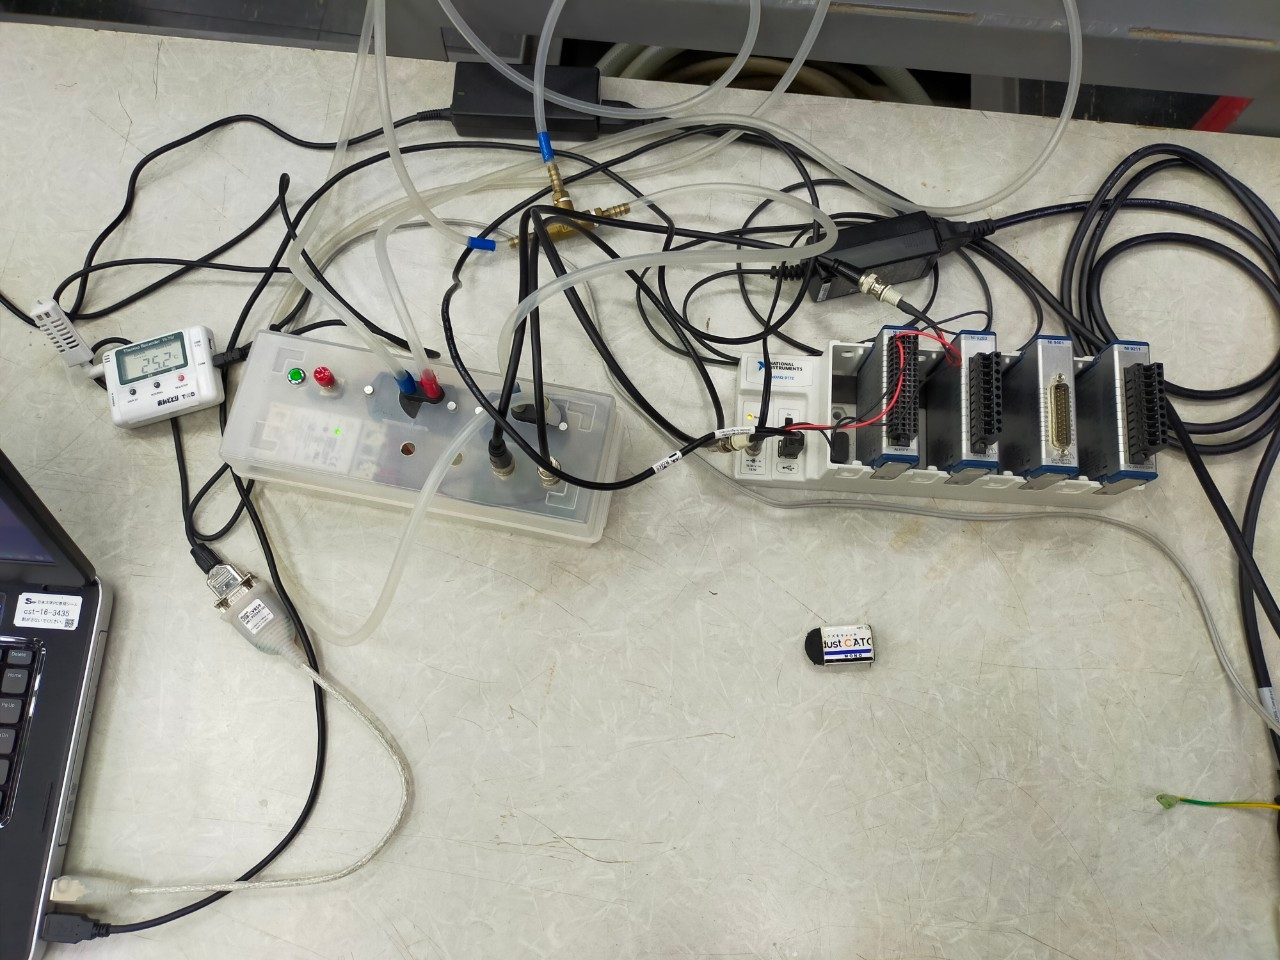
\includegraphics[width=6cm]{すべて.jpg}
  \caption{おんどとり,圧力センサ,A/Dコンバーター}
  \label{すべて}
\end{minipage}
\begin{minipage}[b]{0.45\linewidth}
  \centering
  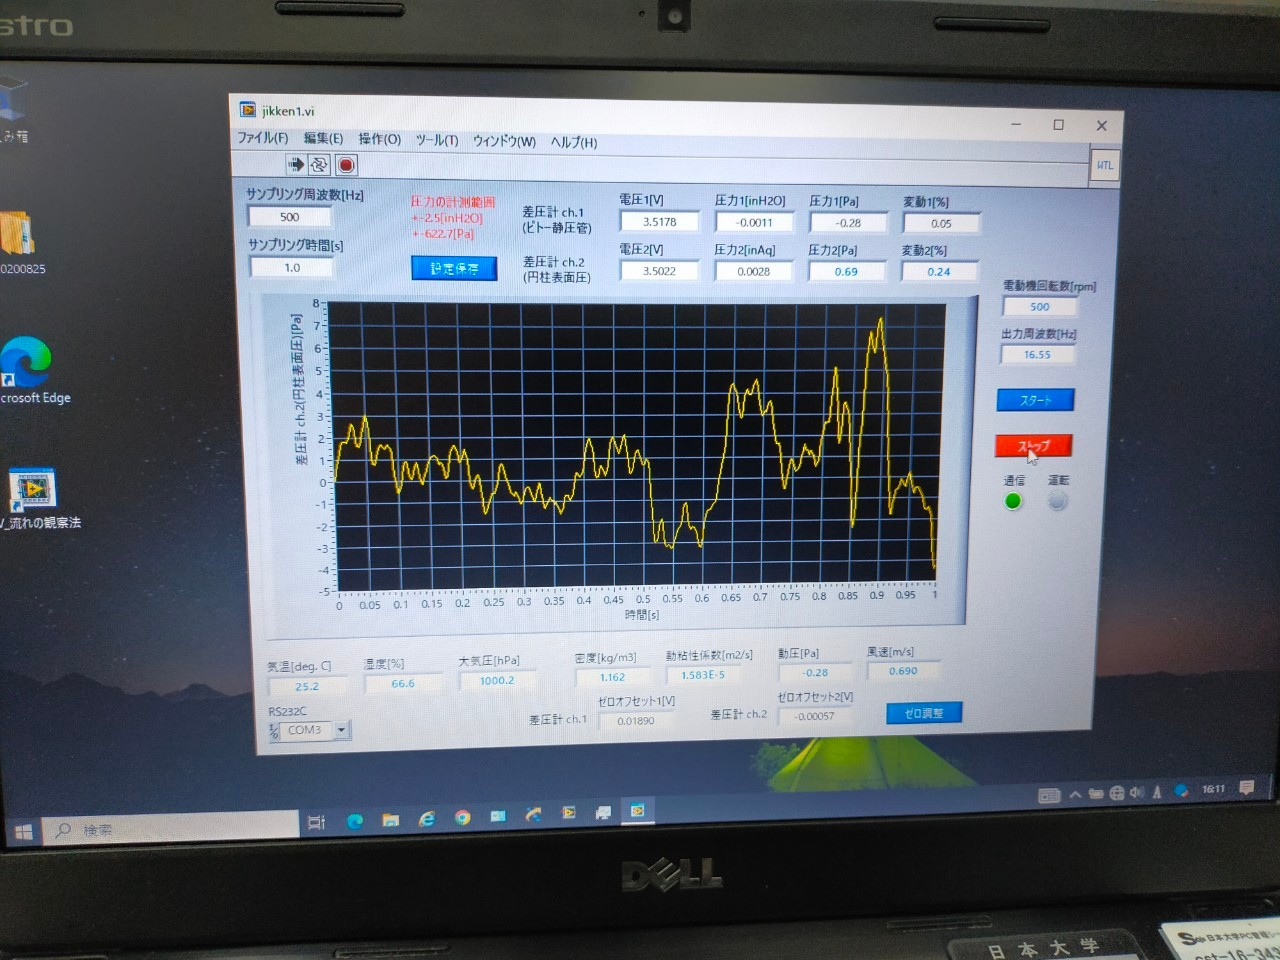
\includegraphics[width=6cm] {pc.jpg}
  \caption{パソコン}
  \label{パソコン}
\end{minipage}
\end{figure}


\begin{table}[hbtp]
  \caption{計測器}
  \centering
  \begin{tabular}{cc}
    \toprule
    計測器\\
    \hline
    おんどとり & 温湿度・大気圧データロガーTANDO Thermo Recorder TR-73U\\
  圧力 & Honeywell圧電抵抗センサー 163Pc01D75 \pm2.5 inH2O (???{\si{Pa}})\\
  パソコン & DELL Vostro 2520 BTX\\
  A/Dコンバーター & 日本ナショナルインスツメンツ DAQ 16bit \pm 10{\si{V}} (分解能???mV)\\
  計測ソフトウェア & 日本ナショナルインスツメンツ LabVIEW\\
  \bottomrule
  \end{tabular}
\end{table}

\section{実験結果}

\subsection{電動機の回転数と測定部の実験結果}

\subsubsection{電動機の回転数と測定部の風速結果}
以下の表は実験前に測定した気象条件である.結果として実験前と実験後では数値はほぼ年化していないことが分かる.

\begin{table}[hbtp]
  \caption{気象条件}
  \centering
  \begin{tabular}{lccc}
    \toprule
    &実験前 & 実験後 & 平均\\
    \hline
    気温{\si{[℃]}} & 24.6 & 25.0 & 24.8\\
  湿度{\si{[\%]}} & 75.2 & 65.6 & 70.4\\
  大気圧 {\si{[hPa]}} & 1000.2 & 1000.0 & 1000.1\\
  密度 {\si{[kg/m^3]}}& 1.163 & 1.162 & 1.1625\\
  動粘性係数 {\si{[m^2/s]}} & $1.578\times10^{-5}$ & $1.581\times10^{-5}$ & $1.5795\times10^{-5}$\\
  \bottomrule
  \end{tabular}
\end{table}

\clearpage

\subsubsection{電動機の回転数と測定部の風速の計測値}
以下の表は回転数ごとに計測した動圧,風速,変動率をまとめたものである.

\begin{table}[hbtp]
  \caption{計測結果}
  \centering
  \begin{tabular}{cccc}
    \toprule
    回転数 & 動圧{\si{[Pa]}} & 風速{\si{[m/s]}} & 変動率{\si{[\%]}}\\
    \hline
    100 & 1.04 & 2.145 & 0.05\\
    200 & 4.87 & 2.739 & 0.04\\
    300 & 10.32 & 4.826 & 0.05\\
    400 & 16.78 & 5.423 & 0.06\\
    500 & 27.98 & 6.855 & 0.05\\
    600 & 44.21 & 8.538 & 0.07\\
    700 & 63.80 & 10.194 & 0.06\\
    800 & 77.35 & 11.561 & 0.06\\
    900 & 98.52 & 12.942 & 0.08\\
    1000 & 122.11 & 14.562 & 0.09\\
    \bottomrule
  \end{tabular}
\end{table}

回転数と風速の関係は以下の図の通りである.

\begin{figure}[hbtp]
  \centering
  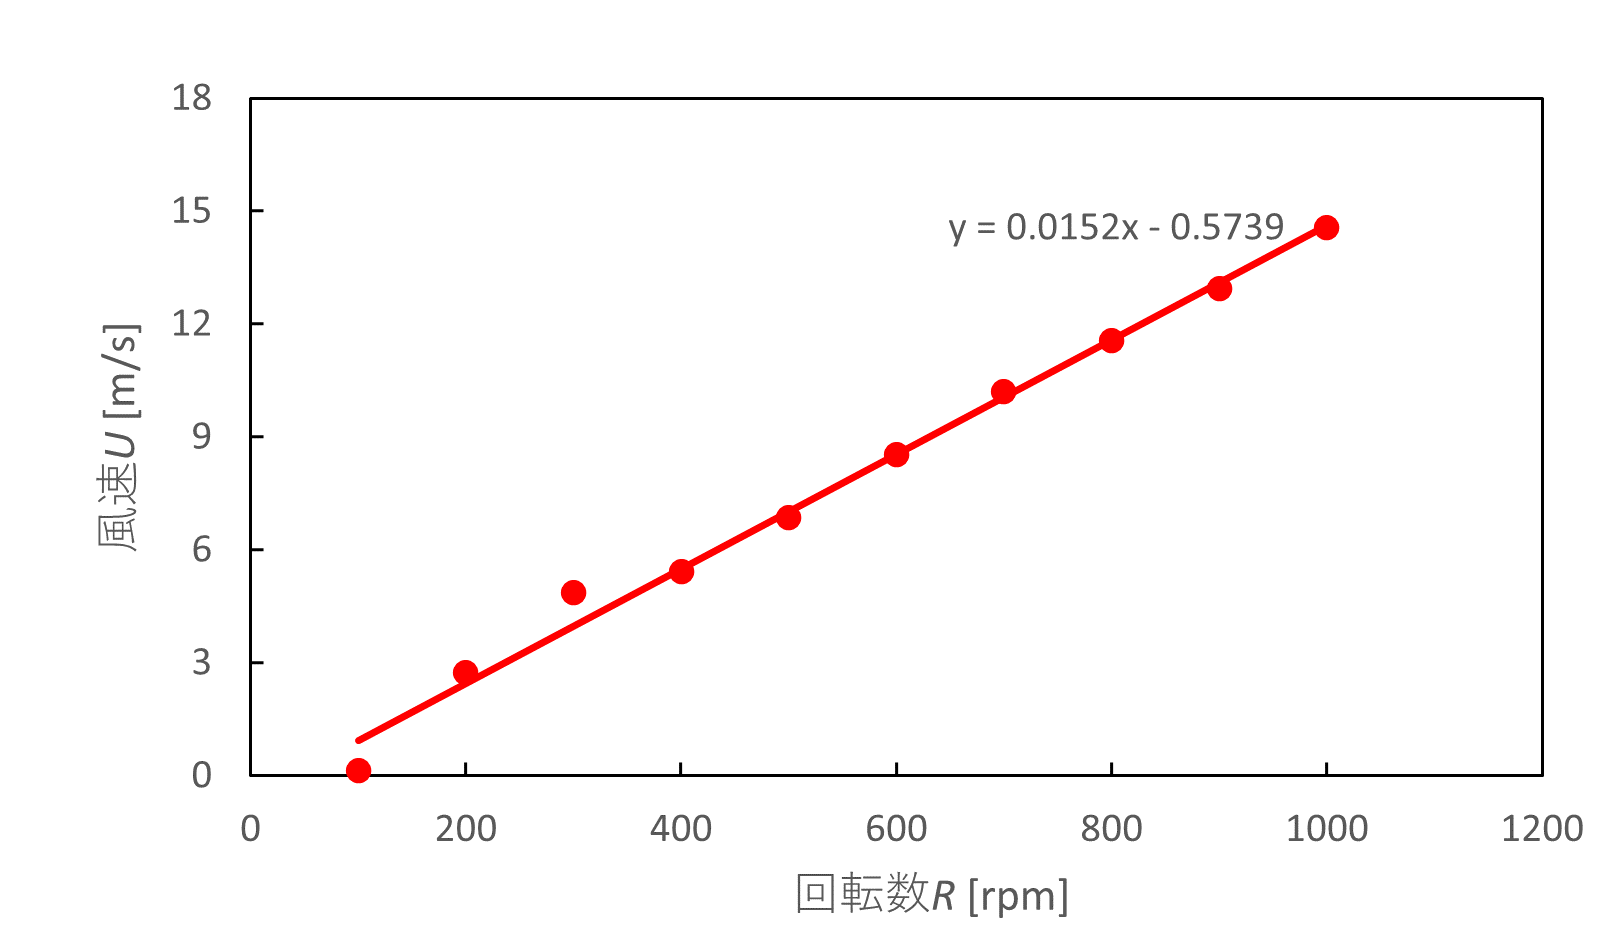
\includegraphics[width=12cm]{回転数と風速.png}
  \caption{回転数と風速の関係}
  \label{回転数と風速}
\end{figure}

図10より,風速4$U$と回転数$R$には比例の関係があることが分かった.

\subsection{円柱の圧力分布の結果}

まず最初に閉塞率を求める.

\begin{equation}
  \text{BR} [\%]=\frac{{\text 円柱の正投影面識}}{\text 測定部の断面積}\times100
\end{equation}

BRは閉塞率を表す.

\begin{equation}
  \frac{30.45\times100}{100}\times100=7.6125\fallingdotseq 7.61 \%
\end{equation}

以下は実験前と実験後の気象条件をまとめたものだ.

\begin{table}[hbtp]
  \caption{気象条件}
  \centering
  \begin{tabular}{lccc}
    \toprule
    &実験前 & 実験後 & 平均\\
    \hline
    気温{\si{[℃]}} &25.1 & 25.4 & 25.25\\
  湿度{\si{[\%]}} & 65.5 & 60.2 & 62.85\\
  大気圧 {\si{[hPa]}} & 1000.0 & 999.9 & 999.5\\
  密度 {\si{[kg/m^3]}}& 1.162 & 1.161 & 1.1615\\
  動粘性係数 {\si{[m^2/s]}} & $1.582\times10^{-5}$ & $1.58\times10^{-5}$ & $1.581\times10^{-5}$\\
  \bottomrule
  \end{tabular}
\end{table}

ここで,レイノルズ数は以下の式で算出する.$U$:風速 $d$:代表長さ \nu :動粘度係数

\begin{equation}
  Re=\frac{Ud}{\nu }\\
  \end{equation}

  計測条件は以下の通りだ.
\begin{table}[hbtp]
  \caption{計測条件}
  \centering
  \begin{tabular}{lc}
    \toprule
    回転数 {\si{[rpm]}}& 1000 \\
    動圧 {\si{[Pa]}} & 121.51\\
  風速 {\si{[m/s]}} & 14.523\\
  円柱の直径 {\si{[mm]}} & 30.45\\
  レイノズル数 {\si{[-]}} & $2.80\times 10^4$\\
  測定部の幅{\si{[mm]}} & 100\\
 測定部の高さ{\si{[mm]}}& 400\\
 閉塞率 {\si{[\%]}} & 7.61\\
 \bottomrule
  \end{tabular}
\end{table}

\clearpage

\subsubsection{円柱の圧力分布の計測値}
\begin{table}[hbtp]
  \caption{計測値}
  \centering
  \begin{tabular}{cccccc}
    \toprule
    角度 {\si{[deg]}}& $P-P_{\infty}$ & 変動率 {\si{[\%]}} & 角度 {\si{[deg]}}& $P-P_{\infty}$ & 変動率 {\si{[\%]}}\\
   \hline
    0 & 120.79 & 0.11 & 100 & -138.56 & 0.84\\
   10 & 103.92 & 0.12 & 110 & -141.64 & 0.87\\
   20 & 75.18 & 0.13 & 120 & -143.16 & 0.99\\
   30 & 11.83 & 0.19 & 130 & -137.12 & 0.8\\
   40 & -51.74 & 0.28 & 140 & -151.94 & 1.14\\
   50 & -108.65 & 0.37 & 150 & -153.81 & 1.35\\
   60 & -154.11 & 0.69 & 160 & -158.97 & 1.63\\
   70 & -162.99 & 0.84 & 170 & -161.47 & 1.87\\
   80 & -144.67 & 1.05 & 180 & -162.54 & 1.91\\
   90 & -142.06 & 0.90&  & &\\
 \bottomrule
  \end{tabular}
\end{table}

上の表から圧力係数$C_P$の算出を行う.
圧力係数$C_P$は次式で定義された.
\begin{equation}
  C_p=\frac{p-p_\infty}{q}=\frac{p-p_\infty}{\frac{\rho U^2}{2}}
\end{equation}

式(9)より,各角度における圧力係数を算出する.

\begin{table}[hbtp]
  \caption{各角度での圧力係数}
  \centering
  \begin{tabular}{cccc}
    \toprule
    角度 {\si{[deg]}}& 圧力係数 $C_P$& 角度 {\si{[deg]}}& 圧力係数$C_P$ \\
    \hline
   0 & 0.986& 100 & -1.13\\
   10 & 0.848& 110 & -1.16\\
   20 & 0.614& 120 & -1.17\\
   30 & 0.0966& 130 & -1.12\\
   40 & -0.422& 140 & -1.24\\
   50 & -0.8877& 150 & -1.26\\
   60 & -1.26& 160 & -1.30\\
   70 & -1.33& 170 & -1.32\\
   80 & -1.18& 180 & -1.33\\
   90 & -1.16&  & \\
 \bottomrule
  \end{tabular}
\end{table}

表10より圧力係数$C_P$をグラフ化すると以下の通りになる.
\clearpage

\begin{figure}[hbtp]
  \centering
  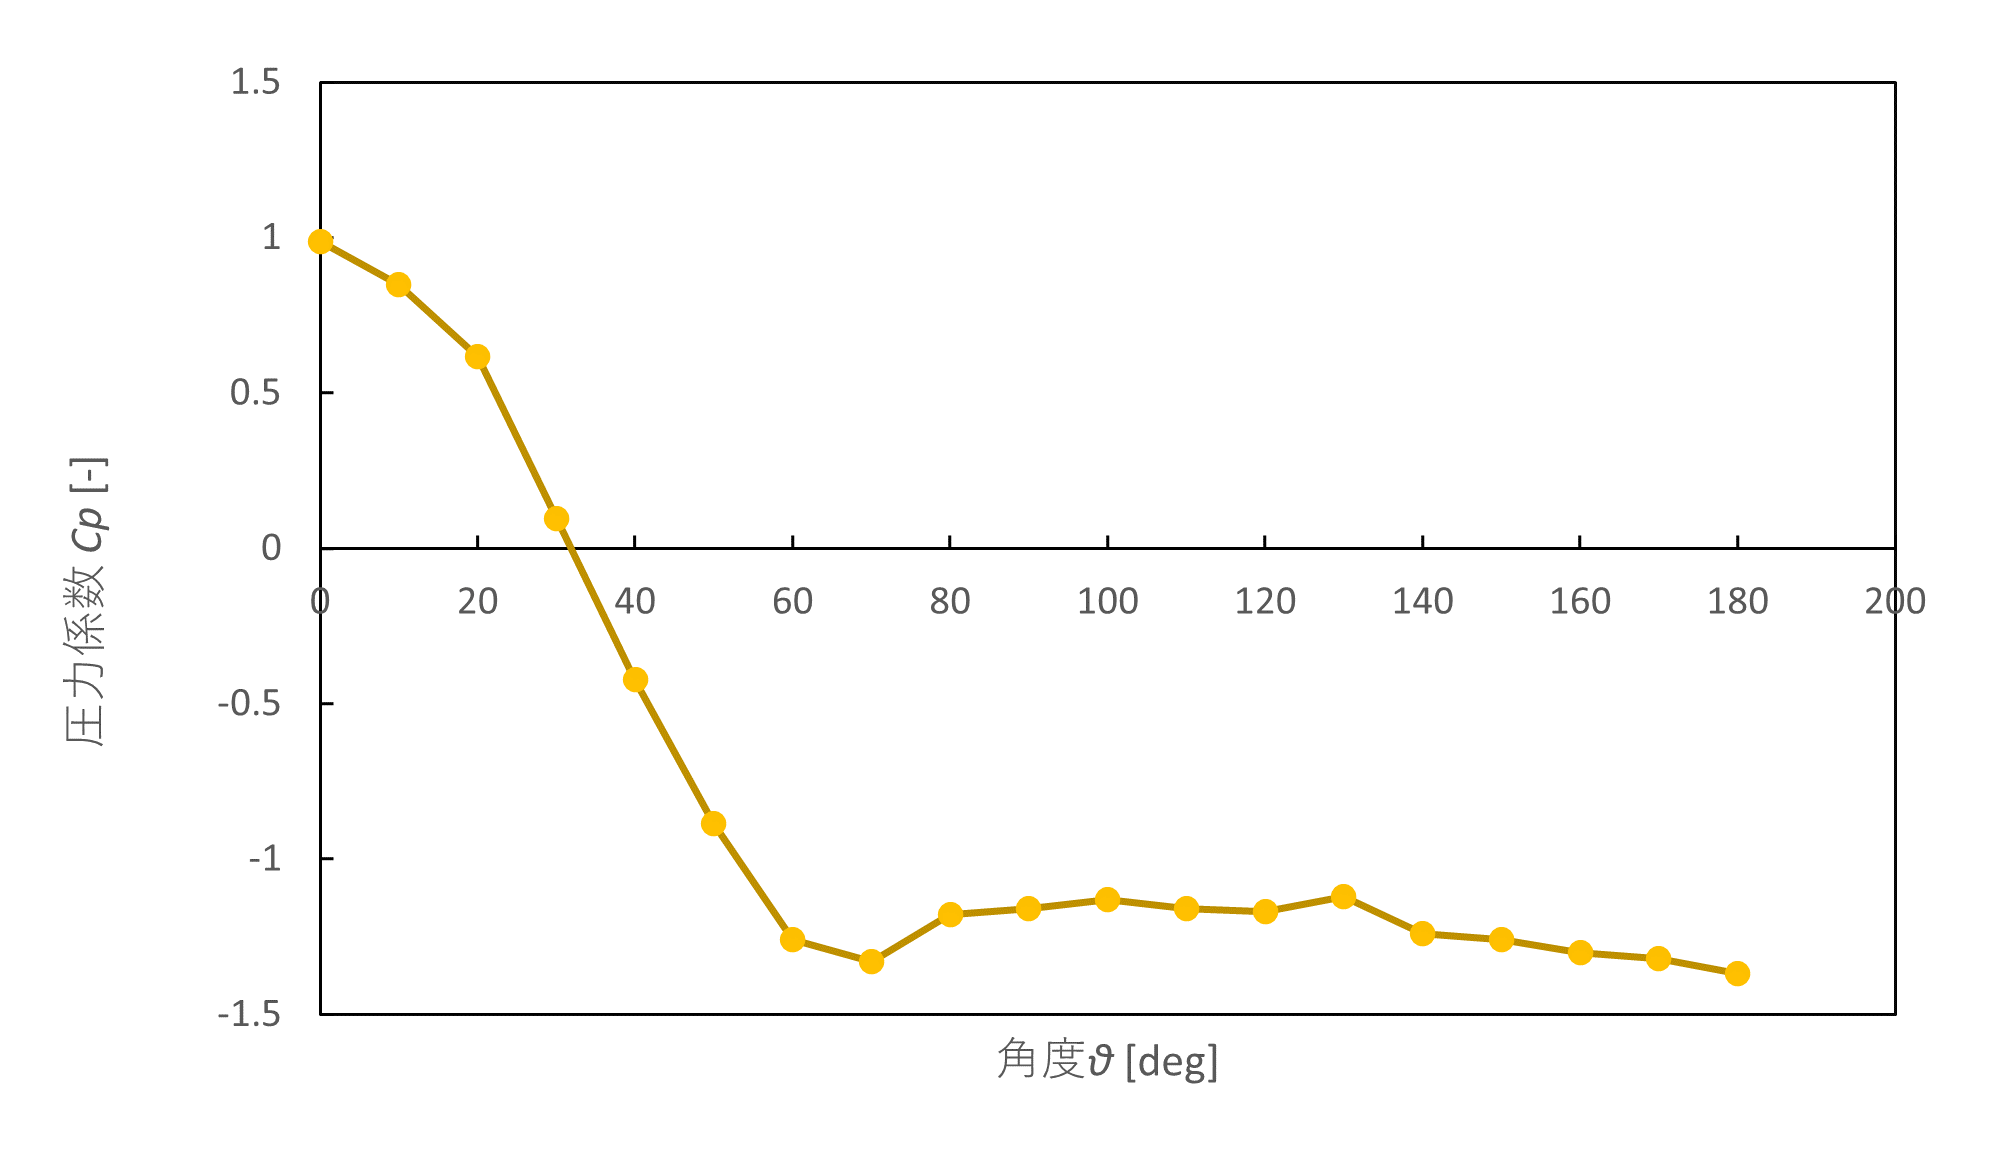
\includegraphics[height=9cm,width=15cm]{圧力係数.png}
  \caption{圧力係数と角度の関係}
  \label{圧力係数}
\end{figure}
圧力係数は$\ang{70}$付近まで三角関数的に推移していき\ang{70}で最小値$-1.33$をと取っていることが表10と図11からわかる

次に,抵抗係数$C_D$を求めるにあたって,$C_P\cos\theta$を算出する.

\begin{table}[hbtp]
  \caption{各角度での圧力係数}
  \centering
  \begin{tabular}{cccc}
    \toprule
    角度 {\si{[deg]}}& $C_P\cos\theta$ & 角度 {\si{[deg]}}& $C_P\cos\theta$ \\
    \hline
   0 & 0.986 & 100 & 0.196\\
   10 & 0.836& 110 & 0.400\\
   20 & 0.577& 120 & 0.584\\
   30 & 0.0840& 130 & 0.720\\
   40 & -0.324& 140 & 0.950\\
   50 & -0.570& 150 & 1.09\\
   60 & -0.629& 160 & 1.22\\
   70 & -0.455& 170 & 1.30\\
   80 & -0.205& 180 & 1.33\\
   90 & -0.00&  & \\
 \bottomrule
  \end{tabular}
\end{table}

表11で求めた$C_P\cos\theta$を用いて2つの算出方法で抵抗係数$C_D$を求める.
\begin{enumerate}
  \item 台形法により数値積分して求める.
  \item シンプソンの公式より数値積分して求める.
\end{enumerate}

\subsubsection{台形法による求め方}
 台形法は区分求積法で発生する誤差をより小さくするために工夫された数値積分の手法である.台形法で求めるにあたって用いる式は以下の通りだ.hは横軸の角度の間隔を表している.今回は18個に分けて考えるため,h=10でる.また,ここでは面積をS'とする.


 \begin{equation}
  S'=\int_{a}^{b} f(x)\,dx =\sum_{n = 0}^{k=18}\frac{h}{2}(f_{k-1}+f_k)
 \end{equation}

 この式から求めた台形の面積は以下の表のとおりだ.
 
\begin{table}[hbtp]
  \caption{台形の面積}
  \centering
  \begin{tabular}{cccc}
    \toprule
    角度 {\si{[deg]}}& 台形の面積 {\si{[m^2]}} & 角度 {\si{[deg]}}& 台形の面積 {\si{[m^2]}} \\
    \hline
   0\sim10 & 9.108 & 100\sim110 & 2.960\\
   10\sim20 & 7.061& 110\sim120 & 4.899\\
   20\sim30 & 3.302& 120\sim130 & 6.520\\
   30\sim40 & -1.200& 130\sim140 & 8.349\\
   40\sim50 & -4.469& 140\sim150 & 10.19\\
   50\sim60 & -5.996& 150\sim160 & 11.54\\
   60\sim70 & -5.421& 160\sim170 & 12.60\\
   70\sim80 & -3.301& 170\sim180 & 13.13\\
   80\sim90 & -1.025& \\
   90\sim100 & 0.982&  & \\
 \bottomrule
  \end{tabular}
\end{table}

表12で算出した台形の面積を足し合わせれば,全体の面積Sが明らかになる.

\begin{equation}
  S=\sum_{n = 1}^{k=18}S =69.2
\end{equation}
となるので,抵抗係数$C_D$は

\begin{equation}
  C_D=\frac{\int _Sp\cos \theta dA}{\frac{\rho U^2S}{2}}=\frac{\pi}{180}\int_{180}^{0} C_p\cos \theta d\theta 
  \label{cd}=\frac{\pi}{180}\times S= 1.208
\end{equation}

\subsubsection{シンプソンの公式による求め方}
閉区間[a,b]を2nで等分すると次の近似式が成り立つ.

\begin{equation}
  S=\int_{a}^{b} f(x) \,dx \fallingdotseq \frac{h}{3}\{ (f_0+f_{2n})+4(f_1+f_3…+f_{2n-1}+2(f_2+f_4+f_{2n-2}))\} 
\end{equation}

hは$\frac{(b-a)}{2n}$で表すことができ,今回はnは9とする.
式(13)を用いて計算をすると
\begin{equation}
  S=\int_{0}^{180}C_P\cos\theta  \,d\theta = 68.77
\end{equation}
よって,式(5)より


\begin{equation}
  C_D=\frac{\int _Sp\cos \theta dA}{\frac{\rho U^2S}{2}}=\frac{\pi}{180}\int_{180}^{0} C_p\cos \theta d\theta 
  \label{cd2}=\frac{\pi}{180}\times S=1.200
\end{equation}
\\
\begin{table}[hbtp]
  \caption{台形法とシンプソンの公式で求めた面積Sと抵抗係数$C_D$}
  \centering
  \begin{tabular}{lcc}
    \toprule
    &面積$S$&抵抗係数$C_D$\\
    \hline
    台形法&69.2&1.207\\
    シンプソンの公式&68.77&1.200\\
    \bottomrule
  \end{tabular}
\end{table}
\\
台形法とシンプソンの公式より$C_P\cos\theta$から$C_D$を求めることができた.
\begin{figure}[hbtp]
  \centering
  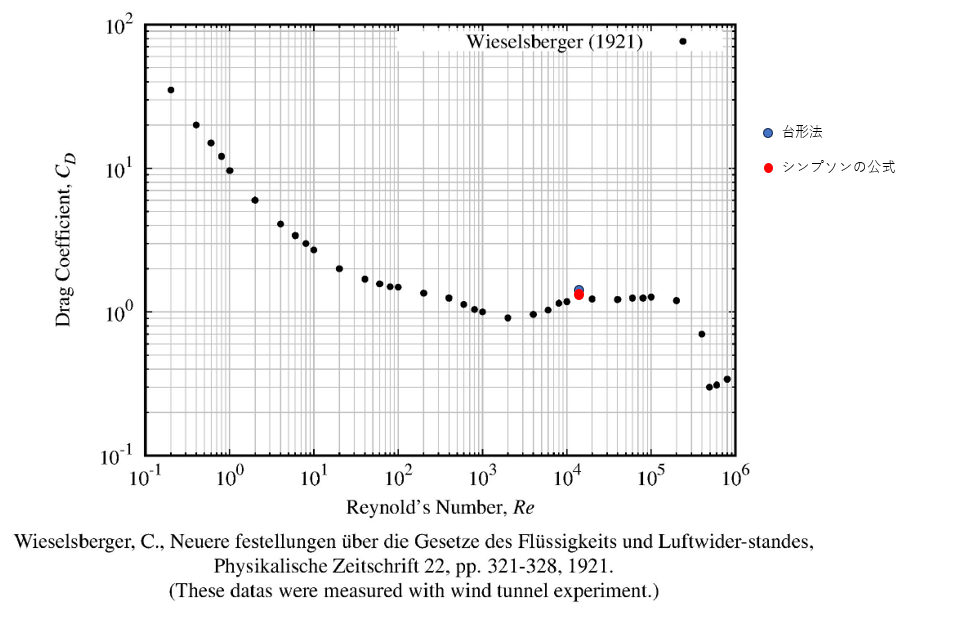
\includegraphics[width=15cm]{図9.png}
  \caption{抵抗係数$C_D$の比較}
  \label{}
\end{figure}

\begin{comment}
<includegraphicsのオプション>
height : 表示画像の高さ指定
width : 表示画像の幅指定
scale : 表示画像の縮尺指定
angle : 表示画像を回転 (単位は度°)
\end{comment}

\clearpage

\subsection{物体まわりの流れの可視化の実験結果}
以下の表に実験時の気象条件,計測条件,各模型の代表さを
,角度範囲,レイノルズ数を示した.

\begin{table}[hbtp]
  \caption{気象条件}
  \centering
  \begin{tabular}{lc}
    \toprule
    &実験前 \\
    \hline
    気温{\si{[℃]}} &25.4\\
  湿度{\si{[\%]}} & 63.6\\
  大気圧 {\si{[hPa]}} & 1000.0\\
  密度 {\si{[kg/m^3]}}& 1.161\\
  動粘性係数 {\si{[m^2/s]}} & $1.585\times10^{-5}$\\
  \bottomrule
  \end{tabular}
\end{table}

\begin{table}[hbtp]
  \caption{計測条件}
  \centering
  \begin{tabular}{lc}
    \toprule
    回転数 {\si{[rpm]}} & 500\\
    動圧 {\si{[Pa]}} & 27.38\\
    風速 {\si{[m/s]}} & 6.990\\
    \bottomrule
  \end{tabular}
\end{table}

\begin{table}[hbtp]
  \caption{模型}
  \centering
  \begin{tabular}{lccc}
    \toprule
    模型 & 代表長さ {\si{[mm]}} & 角度範囲 {\si{[deg]}} & レイノズル数\\
    円柱 & 30.10& - & $1.327\times 10^4$\\
    角柱 & 30.25 &0{ \si{deg}},45{ \si{deg}} &$1.334\times 10^4$\\
    翼型 NACA2418 & 139.90 & -5{ \si{deg}}\sim15{ \si{deg}} & $6.20\times10^5$\\
    \bottomrule
  \end{tabular}
\end{table}

以下に各模型の煙による可視化した流れを示す.
\begin{figure}[hbtp]
  \centering
  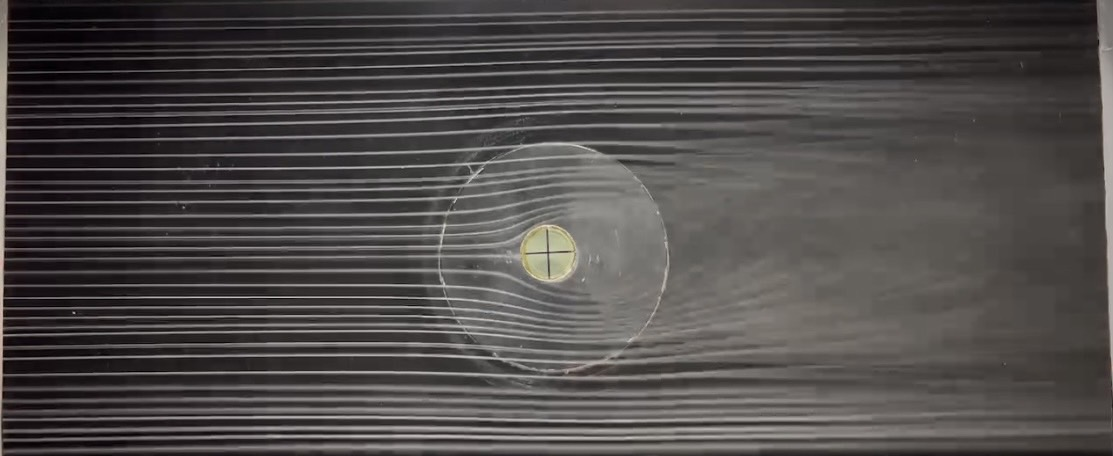
\includegraphics[width=12cm]{円柱周りの流れ.jpg}
  \caption{円柱周りの流れ}
  \label{円柱周りの流れ}
\end{figure}

\begin{figure}[hbtp]
  \centering
  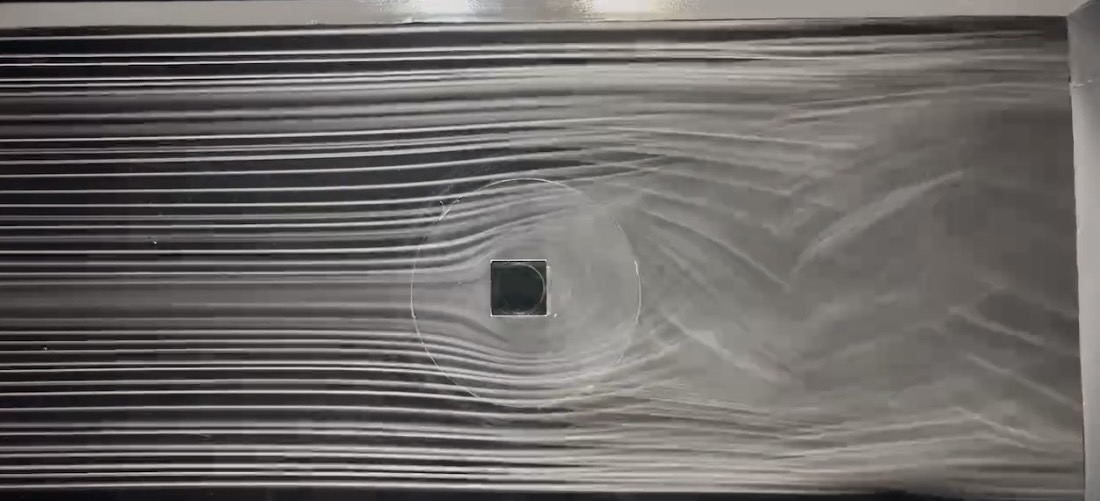
\includegraphics[width=12cm]{角柱0周りの流れ.jpg}
  \caption{角柱(\theta=\ang{0})周りの流れ}
  \label{角柱0}
\end{figure}

\begin{figure}[hbtp]
  \centering
  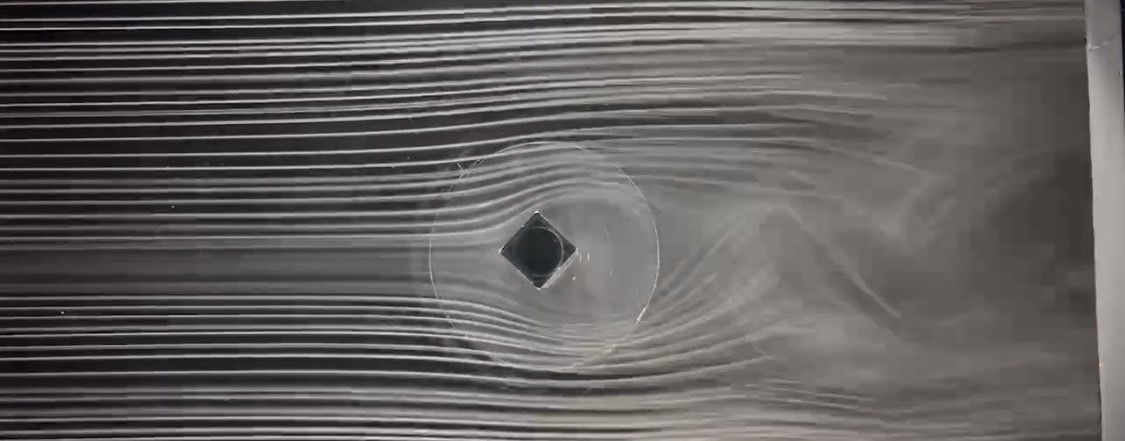
\includegraphics[width=12cm]{角柱45周りの流れ.jpg}
  \caption{角柱(\theta=\ang{45})周りの流れ}
  \label{角柱45}
\end{figure}

\begin{figure}[hbtp]
  \centering
  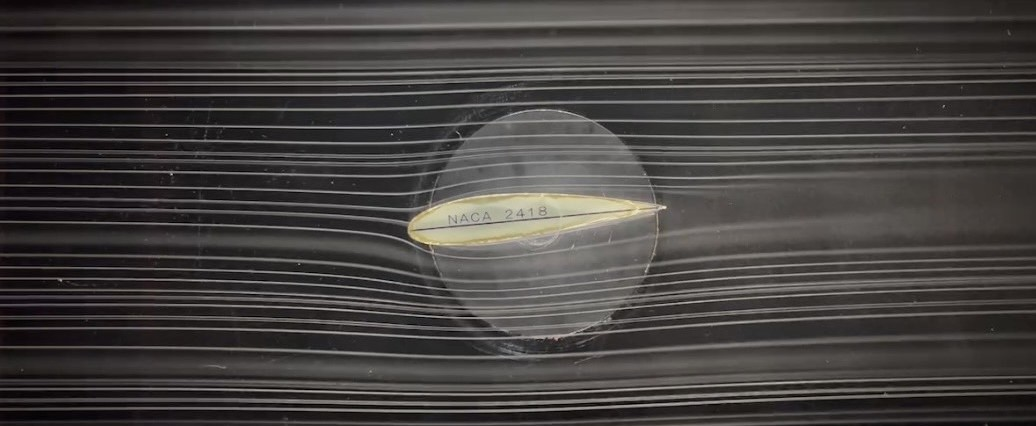
\includegraphics[width=12cm]{翼型模型-5周りの流れ.jpg}
  \caption{翼型模型(\theta=\ang{-5})周りの流れ}
  \label{翼型模型-5}
\end{figure}

\begin{figure}[hbtp]
  \centering
  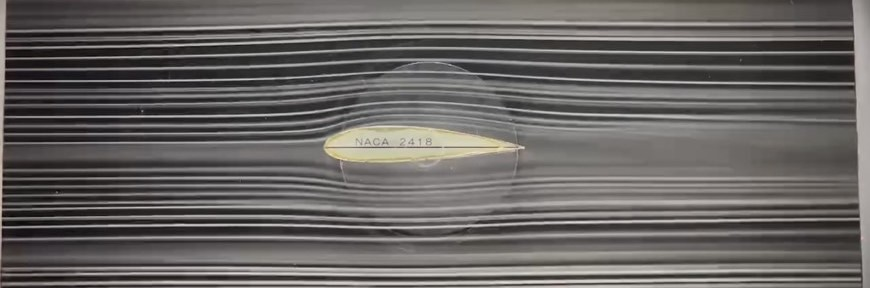
\includegraphics[width=12cm]{翼型模型0周りの流れ.jpg}
  \caption{翼型模型(\theta=\ang{0})周りの流れ}
  \label{翼型模型0}
\end{figure}

\begin{figure}[hbtp]
  \centering
  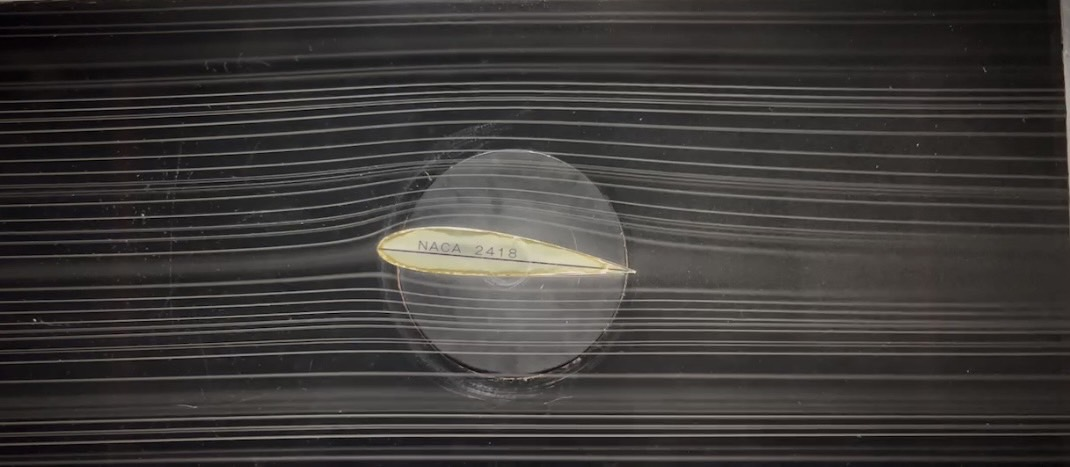
\includegraphics[width=12cm]{翼型模型5周りの流れ.jpg}
  \caption{翼型模型(\theta=\ang{5})周りの流れ}
  \label{翼型模型5}
\end{figure}


\begin{figure}[hbtp]
  \centering
  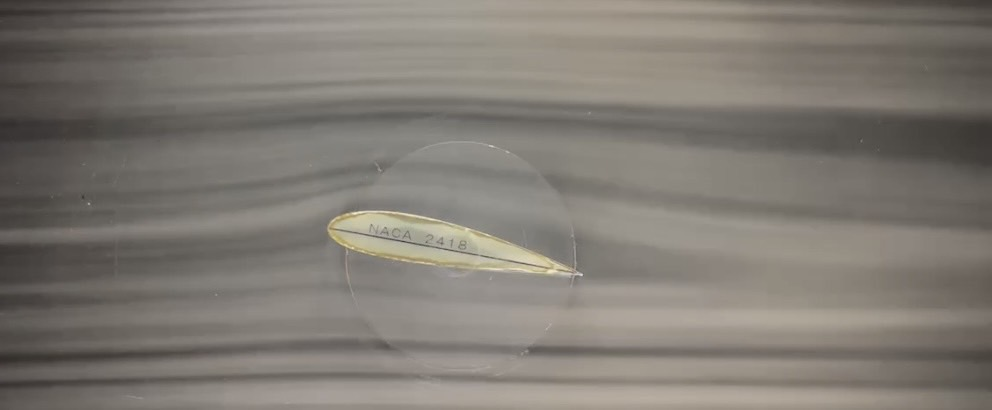
\includegraphics[width=12cm]{翼型模型10周りの流れ.jpg}
  \caption{翼型模型(\theta=\ang{10})周りの流れ}
  \label{翼型模型10}
\end{figure}

\clearpage

\begin{figure}[hbtp]
  \centering
  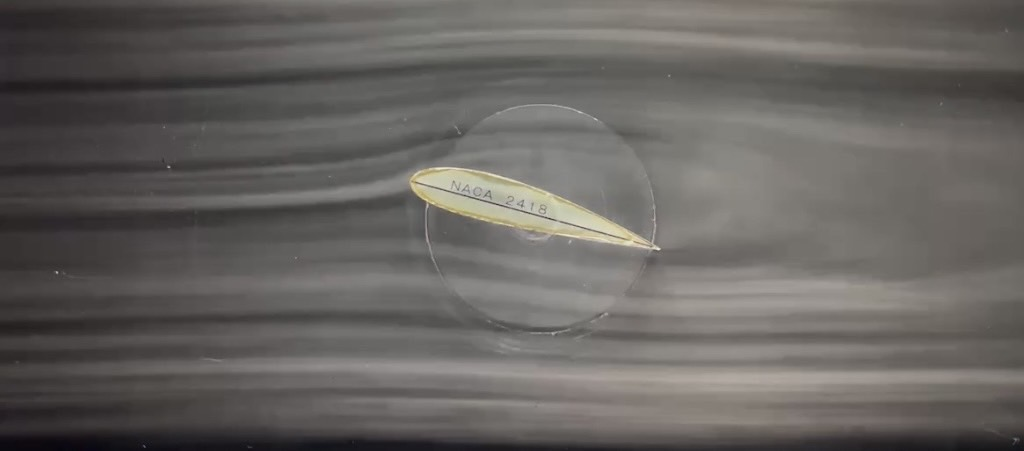
\includegraphics[width=12cm]{翼型模型15周りの流れ.jpg}
  \caption{翼型模型(\theta=\ang{15})周りの流れ}
  \label{翼型模型15}
\end{figure}


\section{考察}
\subsection{電動機の回転数と測定部の風速の計測値}
図10より,回転数$R$が0のとき,yはマイナスになる.これは管摩擦抵抗によるものだ.管摩擦抵抗が作用すると,風洞内の内壁と流体との間には,流れと反対方向に摩擦力が発生するからである.これが測定範囲全体で起きているため,近似曲線を引いたときに,y切片がマイナスになったと考える.また,近似曲線とプロットした値がずれている箇所がある.それはパソコン上で波形を読み取る際に,1秒ごとに更新されるため,正確な平均値を取ることができなかったのが原因だ.これは,計測画面を写真に取るなどして目視より正確に値を読み取り算出する方法が良いと考えた.
表5より,気象条件が実験の前後で変化が少ないことから,送風機の風速気象条件に左右されていないことが分かる.加えて,表6より電送機の回転数を増加させると風速や動圧の値も大きくなっていることが分かった.このことに注目してみると,図11より回転数Rと風速Uには比例の関係があることが明らかである.これは,今回用いた風洞が開放型風洞であるため,大気が直接取り込まれるからだ.よって,回転数を上げると風速が強くなると考えた.さらに,図11でプロットした値では近似曲線からずれている値が数か所あるが,原因としてはパソコン上で波形を読み取る際に,1秒ごとの更新された波形が表示されていたため,その値を正確に読み取ることは困難だった.このようなことから,読み取るときの誤差がプロットがずれた原因だと考えた.


\subsection{$円柱の圧力分布の結果^{[7]}$}
圧力係数は$\ang{70}$付近まで三角関数的に推移していき\ang{70}で最小値$-1.33$をと取っていることが表10と図11からわかる.
図11より,剥離点の推定を行う.剥離は正の圧力勾配を与えると起きる.また,剥離の派生は表面圧力分布を変化させる.これを踏まえて図11を見る.まず,圧力勾配が正になったのは,\ang{70}~\ang{80}だ.次に圧力変化に関しては,\ang{0}から三角関数的に推移していたが\ang{80}付近で,ほぼ一定の値を取り始めた.
このような結果から剥離点は,\ang{80}付近であると考える.
今回の実験で得られたデータ図12を見てみると圧力係数$C_P$は$\ang{0}$から三角
関数的に推移していき$\ang{70}$で最小値を取っている.それ以降,\ang{90}まで少し増加し,一定の値になっている.これは,剥離により,圧力が低くなったため,周囲から力が働いたからであると考えられる.また,周囲からの力は抵抗力として働いた.よって,図12を見てみると抵抗係数が増加している$\ang{70}$\thicksim $\ang{90}$付近が剥離点であると推測できる.また,剥離が起きると円柱表面に沿って流れることが不可能になるので,値はほぼ一定になったと考えた.以下に理想流体と実験で得たデータを示す.

\begin{figure}[hbtp]
  \centering
  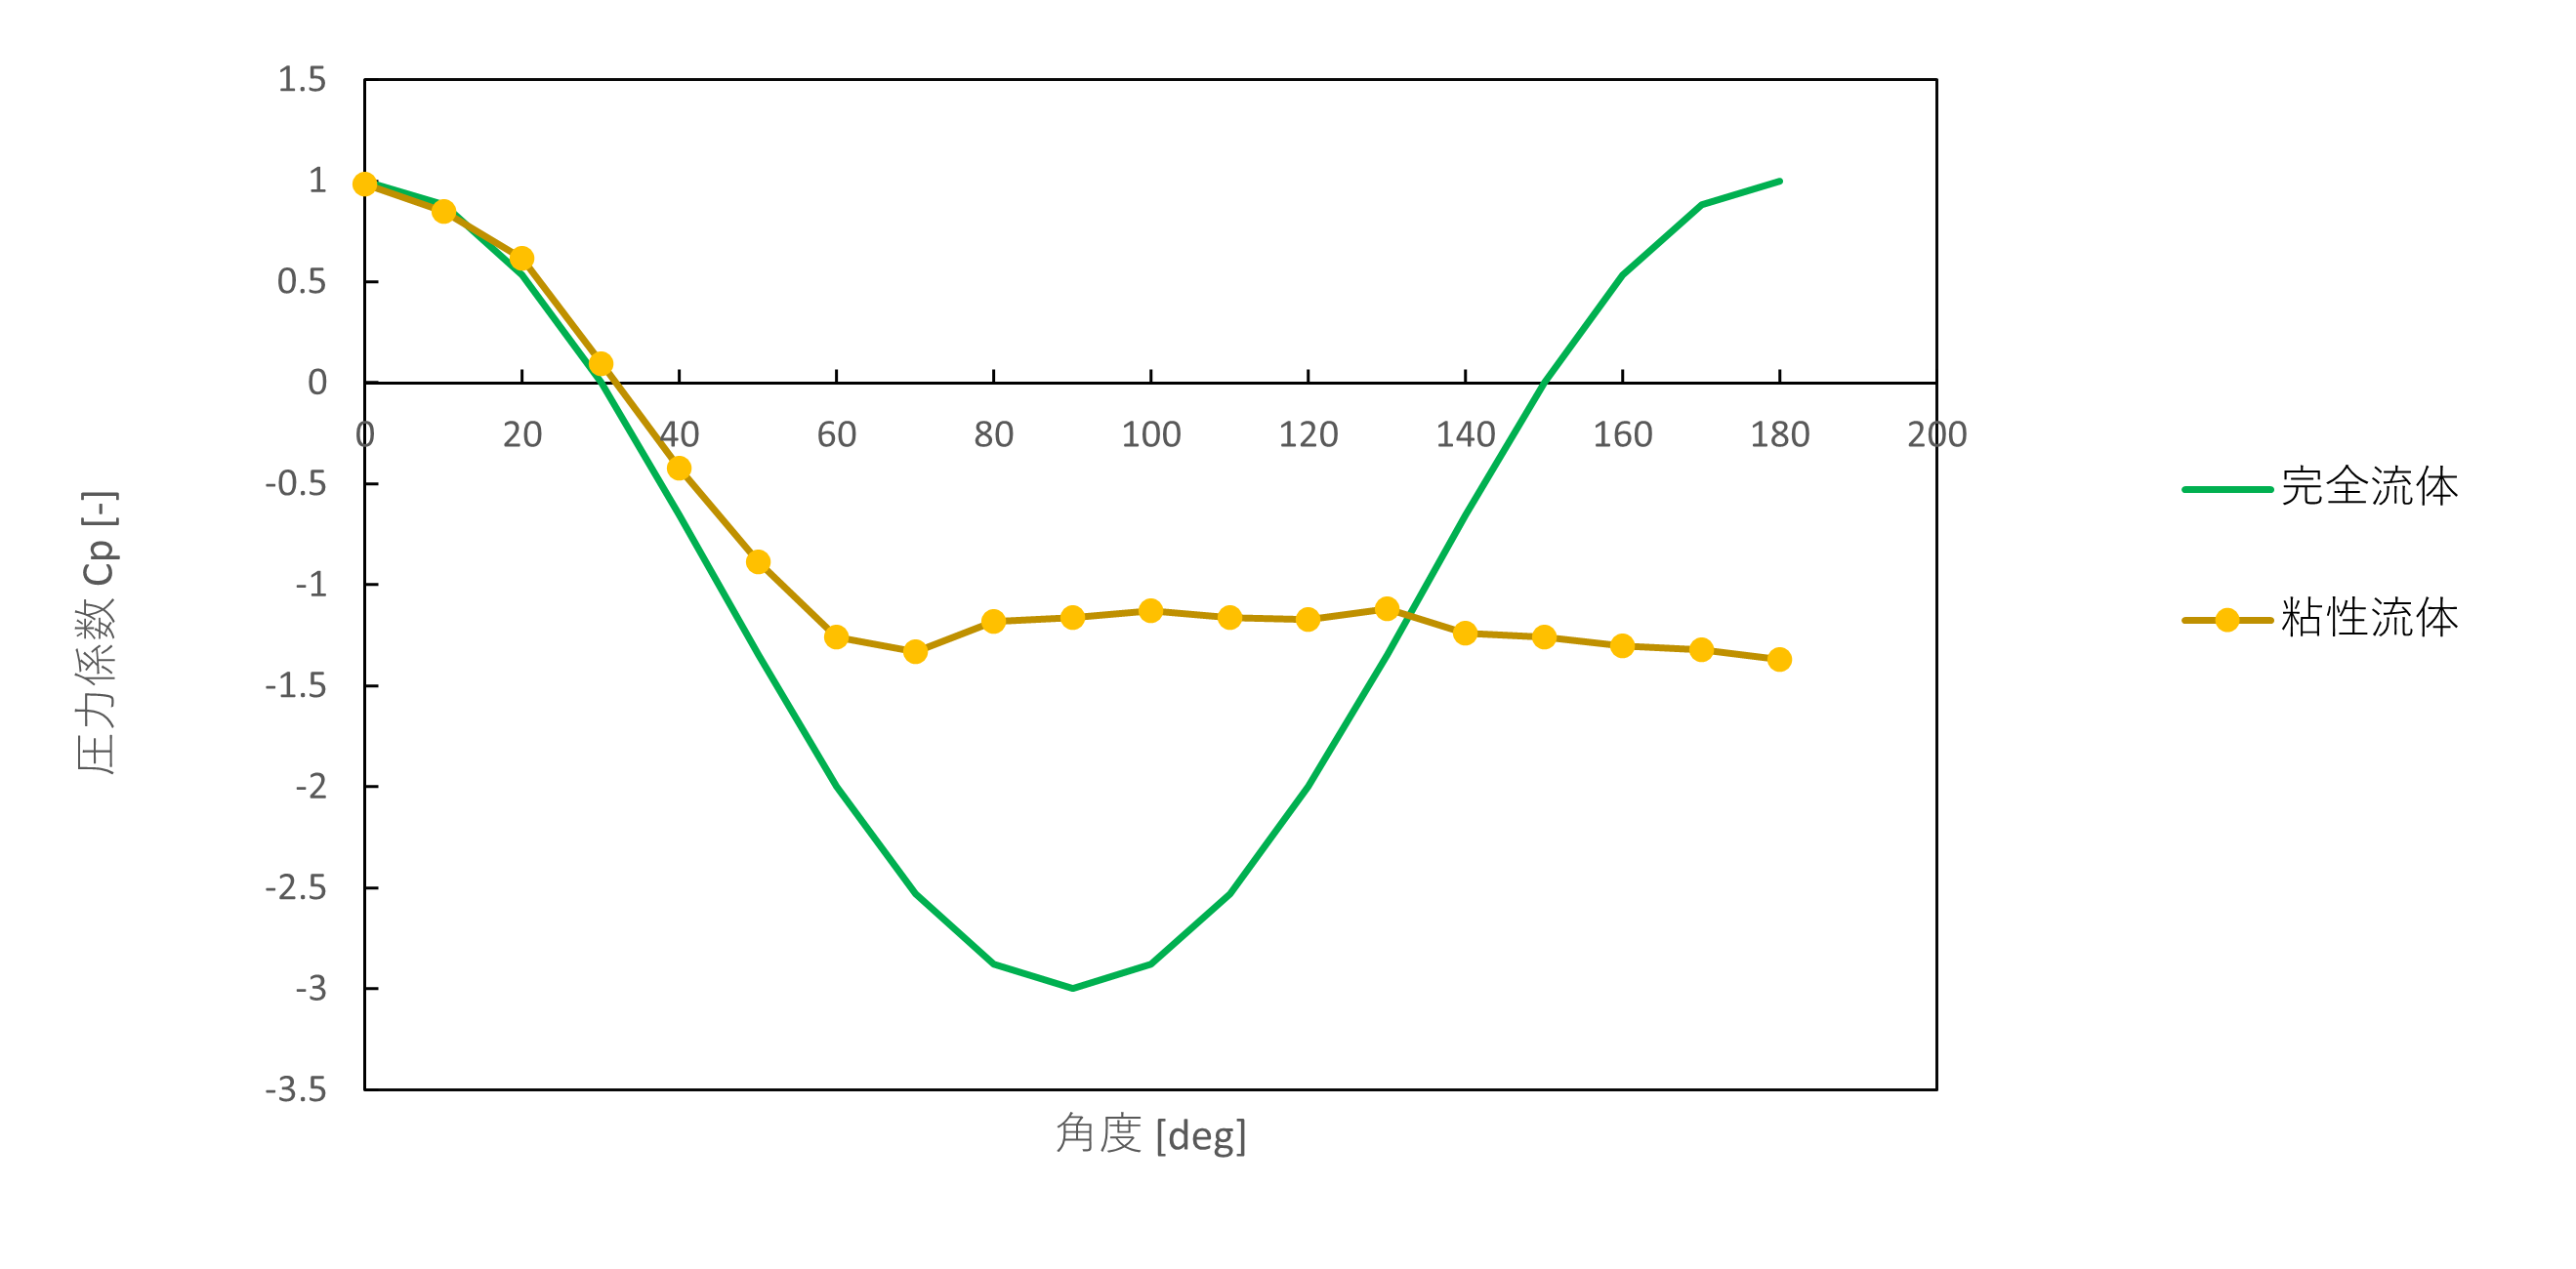
\includegraphics[width=13cm]{圧力係数と角度.png}
  \caption{理想流体の圧力係数と実験値の関係}
  \label{cp}
\end{figure}
理想流体では,粘性,空気抵抗が考慮されていないため,円柱まわり流れは上下対称になり,境界層は発生しない.よって,綺麗な曲線になっていると考えられる.一方で今回の流体では$Re$は$2.80\times10^4$であり,一般的に円柱周りの臨海レイノズル数は$2.0\times10^5$であるため,層流であり,層流境界層が形成されたと考えられる.
よって,理想流体と比較したときに異なる形状のグラフになった推測した.
この実験では,台形法とシンプソンの公式を用いて抵抗係数$C_D$を求めた.台形法はグラフを折れ線グラフにして台形の面積で求め,シンプソンの公式はデータを微小区間で放物線に近似して抵抗係数を算出した.表13よりどちらからほぼ同じ値が求められた.
データの量などで適切に使い分けるのが良いと考える.


\subsection{$物体まわりの流れの可視化^{[1][3]}$}
 図13より,円柱周りの流れは,円柱の断面を単位円として考えたとき,$\frac{\pi}{2}$の付近で流れが乱れ始めていることが分かる.流れがまともにあたる$\pi$の部分では圧力が最も高く,それ以降表面に沿って圧力は減少していき,$\frac{\pi}{2}$で圧力の最小値を取る.しかし,0に行くにつれて増加していく.圧力勾配について考えてみると,$\pi$から時計回りに$\frac{\pi}{2}$をたどると,圧力勾配は負(マイナス)である.一方で,$\frac{\pi}{2}$から時計回りに0までたどると,圧力は増加するため,圧力勾配は正で登り坂になることが分かる.境界層内の流体はの流体は粘性摩擦を受けるため,運動エネルギーを消費することから,次第に速度が遅くなり,0の位置までたどりつくことができず,途中の箇所で静止し,逆流が生じてしまう.その後,模型の後ろ側に渦ができているのが確認できた.これはカルマン渦と呼ばれるもので,流体が模型を通過したしたことで,模型の後方で流速が遅くなって形成されていると考えた.また,カルマン渦列は,物体からの剥離剪断層が主流と直角方向に振動し,その1周期ごとに反対符号の渦が放出されるので,物体の下流に互い違いに並んだ渦ができる.この減少は各角柱(\theta=0°,45°)でも同じ現象が確認できる.
 翼型模型では,空気は物体のまわりを流れるとき,物体の摩擦などから小さな渦を生じ,流れるにしたがってその渦も大きくなり物体の表面に沿いきれず剥離してしまう状況がある.本実験では\theta=15°で明らかに確認できる.
 角度を大きくとった\theta=15°では前縁で剥離が起きていることから,圧力抵抗が増加し,揚力が減少している状態.つまり,前縁失速しているということを意味している.翼の理想の流れとしては翼の表面に均一に流れがあることだ.

 \clearpage
\begin{thebibliography}{99}
%bibitem{キー} 出版社・著者 『[第○版] 題名』,(出版年)
  \bibitem{a} コロナ社・ルードウィヒ・プラントル『流れ学(下)』,(昭和50年)
%bibitem{キー} 著者 『題名』,url{URL},(閲覧日)

  \bibitem{a} 木村秀政『航空用語辞典』,(昭和56年 7月15日)
  \bibitem{a}コロナ社・新藤章二郎『低速風洞実験法』(1992)
  \bibitem{a}理工学社・生井武文,井上雅弘『粘性流体の力学』
  \bibitem{a}朝倉書店,流れの可視化学会『流れの可視化ハンドブック』(1986)
  %bibitem{キー} 出版社・著者 『[第○版] 題名』,(出版年)
    \bibitem{a} 理工学社・松尾一泰『流体の力学』,(2007.10.30)
  %bibitem{キー} 著者 『題名』,url{URL},(閲覧日
  
  
\end{thebibliography}




\end{document}